\PassOptionsToPackage{unicode=true}{hyperref} % options for packages loaded elsewhere
\PassOptionsToPackage{hyphens}{url}
\PassOptionsToPackage{dvipsnames,svgnames*,x11names*}{xcolor}
%
\documentclass[10pt,]{krantz}
\usepackage{lmodern}
\usepackage{amssymb,amsmath}
\usepackage{ifxetex,ifluatex}
\usepackage{fixltx2e} % provides \textsubscript
\ifnum 0\ifxetex 1\fi\ifluatex 1\fi=0 % if pdftex
  \usepackage[T1]{fontenc}
  \usepackage[utf8]{inputenc}
  \usepackage{textcomp} % provides euro and other symbols
\else % if luatex or xelatex
  \usepackage{unicode-math}
  \defaultfontfeatures{Ligatures=TeX,Scale=MatchLowercase}
    \setmonofont[Mapping=tex-ansi,Scale=0.7]{Source Code Pro}
\fi
% use upquote if available, for straight quotes in verbatim environments
\IfFileExists{upquote.sty}{\usepackage{upquote}}{}
% use microtype if available
\IfFileExists{microtype.sty}{%
\usepackage[]{microtype}
\UseMicrotypeSet[protrusion]{basicmath} % disable protrusion for tt fonts
}{}
\IfFileExists{parskip.sty}{%
\usepackage{parskip}
}{% else
\setlength{\parindent}{0pt}
\setlength{\parskip}{6pt plus 2pt minus 1pt}
}
\usepackage{xcolor}
\usepackage{hyperref}
\hypersetup{
            pdftitle={Ecuaciones diferenciales ordinarias},
            pdfauthor={Ricardo Michel MALLQUI BAÑOS},
            colorlinks=true,
            linkcolor=Maroon,
            filecolor=Maroon,
            citecolor=Blue,
            urlcolor=Blue,
            breaklinks=true}
\urlstyle{same}  % don't use monospace font for urls
\usepackage{longtable,booktabs}
% Fix footnotes in tables (requires footnote package)
\IfFileExists{footnote.sty}{\usepackage{footnote}\makesavenoteenv{longtable}}{}
\setlength{\emergencystretch}{3em}  % prevent overfull lines
\providecommand{\tightlist}{%
  \setlength{\itemsep}{0pt}\setlength{\parskip}{0pt}}
\setcounter{secnumdepth}{5}

% set default figure placement to htbp
\makeatletter
\def\fps@figure{htbp}
\makeatother

\usepackage[spanish,es-lcroman]{babel}
\usepackage{booktabs}
\usepackage{graphicx}
\usepackage{amsmath}
\usepackage{makeidx}
\makeindex
%\usepackage{showframe}
%\usepackage[a4paper]{geometry}
%\geometry{verbose,tmargin=3cm,bmargin=3cm,lmargin=3.5cm,rmargin=3cm}
\renewcommand{\arraystretch}{1.1}

\usepackage{times}
\renewcommand{\rmdefault}{ptm}
\usepackage[lite,subscriptcorrection,nofontinfo,zswash]{mtpro2}

\usepackage{graphicx}

% Determine if the image is too wide for the page.
\makeatletter
\def\ScaleIfNeeded{%
  \ifdim\Gin@nat@width>\linewidth
    \linewidth
  \else
    \Gin@nat@width
  \fi
}
\makeatother

% Resize figures that are too wide for the page.
\let\oldincludegraphics\includegraphics
\renewcommand\includegraphics[2][]{%
  \oldincludegraphics[scale=0.85]{#2}
}

\usepackage{amsthm}
\makeatletter
\def\thm@space@setup{%
  \thm@preskip=8pt plus 2pt minus 4pt
  \thm@postskip=\thm@preskip
}
\makeatother



\flushbottom 

\frontmatter
\usepackage[]{natbib}
\bibliographystyle{apalike}

\title{Ecuaciones diferenciales ordinarias}
\author{Ricardo Michel MALLQUI BAÑOS}
\providecommand{\institute}[1]{}
\institute{Universidad Nacional San Cristóbal De Huamanga}
\date{2020-03-28}

\usepackage{amsthm}
\newtheorem{theorem}{Teorema}[chapter]
\newtheorem{lemma}{Lema}[chapter]
\newtheorem{corollary}{Corolario}[chapter]
\newtheorem{proposition}{Proposición}[chapter]
\newtheorem{conjecture}{Conjectura}[chapter]
\theoremstyle{definition}
\newtheorem{definition}{Definición}[chapter]
\theoremstyle{definition}
\newtheorem{example}{Ejemplo}[chapter]
\theoremstyle{definition}
\newtheorem{exercise}{Ejercicio}[chapter]
\theoremstyle{remark}
\newtheorem*{remark}{Observación}
\newtheorem*{solution}{Solución}
\let\BeginKnitrBlock\begin \let\EndKnitrBlock\end
\begin{document}
\maketitle

%\cleardoublepage\newpage\thispagestyle{empty}\null
%\cleardoublepage\newpage\thispagestyle{empty}\null
%\cleardoublepage\newpage
\thispagestyle{empty}
\begin{center}
\includegraphics{U.pdf}
\end{center}

%\setlength{\abovedisplayskip}{-5pt}
%\setlength{\abovedisplayshortskip}{-5pt}

{
\hypersetup{linkcolor=}
\setcounter{tocdepth}{2}
\tableofcontents
}
\listoftables
\listoffigures
\newcommand{\N}{\mathbb{N}}
\newcommand{\R}{\mathbb{R}}
\newcommand{\CC}{\mathbb{C}}
\newcommand{\I}{\mathbb{I}}
\newcommand{\f}{\mathbb{f}}
\newcommand{\X}{\mathbb{X}}
\newcommand{\D}{\mathbb{D}}
\newcommand{\Z}{\mathbb{Z}}
\newcommand{\Q}{\mathbb{Q}}
\newcommand{\norm}[1]{\left\Vert#1\right\Vert}
\newcommand{\abs}[1]{\left\vert#1\right\vert}
\newcommand{\set}[1]{\left\{#1\right\}}
\newcommand{\seq}[1]{\left<#1\right>}
\newcommand{\co}[1]{\left[#1\right]}
\newcommand{\cc}[1]{\left(#1\right)}
\newcommand{\J}{\mathcal{J}}
\newcommand{\K}{\mathcal{K}}
\newcommand{\M}{\mathcal{M}}
\newcommand{\F}{\mathcal{F}}

\hypertarget{resumen}{%
\chapter*{Resumen}\label{resumen}}


Este libro sobre ecuaciones diferenciales ordinarias y sus aplicaciones cuyo objetivo es demostrar resultados basicos muy útiles en el desarrollo de investigaciones.

\[\sum_1^2\]

\hypertarget{introducciuxf3n}{%
\chapter*{Introducción}\label{introducciuxf3n}}


\[\sum_1^2\]

\[\vec{u}=(1,1)-\rho\int_2^3\]

Debido a la poca información estructurada de estadistica descriptiva se propone escribir este libro con un enfoque demostrativo.

\[x^2+y^2\]

\mainmatter

\hypertarget{ecuaciones-diferenciales-de-primer-orden-y-primer-grado}{%
\chapter{Ecuaciones diferenciales de primer orden y primer grado}\label{ecuaciones-diferenciales-de-primer-orden-y-primer-grado}}

\begin{align*}
  5&=6\\
  &=7
\end{align*}
Una ecuación ordinaria de primer orden y primer grado se representa como \[F\left(x,y,\frac{dy}{dx}\right)=0\] donde \(F\) relaciona tres variables; una funcion \(y\) su variable independiente \(x\) y su derivada \(\frac{dy}{dx}\), por ejemplo \(\left(y^2+xy^2\right)\frac{dy}{dx}+x^2-x^2y=0\). Si se despeja \(\frac{dy}{dx}\) de \(F\left(x,y,\frac{dy}{dx}\right)=0\) obtenemos \(\frac{dy}{dx}=g(x,y)\).

\hypertarget{ecuaciones-diferenciales-de-variable-separable}{%
\section{Ecuaciones diferenciales de variable separable}\label{ecuaciones-diferenciales-de-variable-separable}}

Si una ecuación ordinaria de primer orden y primer grado \(\frac{dy}{dx}=f(x,y)\) se puede expresarse como \(M(x)dx+N(y)dy=0\) entonces la ecuación recibe el nombre de ecuación diferencial ordinaria de variable separable y la solución es por integración directa \[\int M(x)dx+\int N(y)dy=0\]

\BeginKnitrBlock{exercise}
\protect\hypertarget{exr:unnamed-chunk-1}{}{\label{exr:unnamed-chunk-1} }\(\left(y^2+xy^2\right)\frac{dy}{dx}+x^2-x^2y=0\)
\EndKnitrBlock{exercise}

\BeginKnitrBlock{solution}
\iffalse{} {Solución. } \fi{}\begin{align*}
0&=y^2\left(1+x\right)dy+x^2\left(1-y\right)dx\\
&=\frac{y^2}{1-y}dy+\frac{x^2}{1+x}dx
\end{align*}

integrando se tiene \[\int\frac{y^2}{1-y}dy+\int\frac{x^2}{1+x}dx=\int 0\]
\[(x+y)(x-y-2)+2\ln\left\vert\frac{1+x}{1-y}\right\vert=k\]
\EndKnitrBlock{solution}

\BeginKnitrBlock{exercise}
\protect\hypertarget{exr:unnamed-chunk-3}{}{\label{exr:unnamed-chunk-3} }\(\left(y^2+xy^2\right)\frac{dy}{dx}+x^2-x^2y=0\)
\EndKnitrBlock{exercise}

\BeginKnitrBlock{solution}
\iffalse{} {Solución. } \fi{}\begin{align*}
0&=y^2\left(1+x\right)dy+x^2\left(1-y\right)dx\\
&=\frac{y^2}{1-y}dy+\frac{x^2}{1+x}dx
\end{align*}

integrando se tiene \[\int\frac{y^2}{1-y}dy+\int\frac{x^2}{1+x}dx=\int 0\]
\[(x+y)(x-y-2)+2\ln\left\vert\frac{1+x}{1-y}\right\vert=k\]
\EndKnitrBlock{solution}

\hypertarget{ecuaciones-diferenciales-reducible-a-variable-separable}{%
\section{Ecuaciones diferenciales reducible a variable separable}\label{ecuaciones-diferenciales-reducible-a-variable-separable}}

Ecuaciones de la forma
\begin{equation}
\frac{dy}{dx}=f(ax+by+c)\label{eq:er1}
\end{equation}
donde \(ax+by+c\) es la ecuacion de una recta sobre el plano euclideo son reducibles a variables separables. Si se realiza la sustitución de la derivada de \(z=ax+by+c\) en la ecuación \eqref{eq:er1} se obtiene una ecuación de variable separable. En efecto de \(z=ax+by+c\) se tiene \(\frac{dy}{dx}=\frac{1}{b}\left(\frac{dz}{dx}-a\right)\) esto en \eqref{eq:er1} genera \(\frac{1}{b}\left(\frac{dy}{dx}-a\right)=f(z)\) que es una ecuacion de variable separable \[\frac{dy}{a+bf(z)}=dx.\]

\hypertarget{ecuaciones-diferenciales-homoguxe9neas}{%
\section{Ecuaciones diferenciales homogéneas}\label{ecuaciones-diferenciales-homoguxe9neas}}

\BeginKnitrBlock{definition}
\protect\hypertarget{def:unnamed-chunk-5}{}{\label{def:unnamed-chunk-5} }Una función \(f(x,y)\) es \textbf{homogenea} de \textbf{grado} \(k\) si verifica \[f\left(\lambda x, \lambda y\right)=\lambda^kf(x,y)\]
\EndKnitrBlock{definition}

\begin{verbatim}
\end{verbatim}

\hypertarget{ecuaciones-diferenciales-reducible-a-homoguxe9neas}{%
\section{Ecuaciones diferenciales reducible a homogéneas}\label{ecuaciones-diferenciales-reducible-a-homoguxe9neas}}

\hypertarget{ecuaciones-diferenciales-exactas}{%
\section{Ecuaciones diferenciales exactas}\label{ecuaciones-diferenciales-exactas}}

\hypertarget{ecuaciones-diefrenciales-lineales-de-primer-orden}{%
\section{Ecuaciones diefrenciales lineales de primer orden}\label{ecuaciones-diefrenciales-lineales-de-primer-orden}}

\hypertarget{ecuaciones-diefrenciales-de-bernoulli}{%
\section{Ecuaciones diefrenciales de Bernoulli}\label{ecuaciones-diefrenciales-de-bernoulli}}

Son de la forma
\begin{equation}
\frac{dy}{dx}+p(x)y+q(x)y^{2}=f(x)
\label{eq:w1w}
\end{equation}

La ecuación se resuelve si solo se conoce una solución particular \(y_{1}(x)\). Conocida dicha solución, se hace el cambio
\begin{equation}
y(x)=z(x)+y_{1}(x)
\label{eq:w2}
\end{equation}
despejando \(\frac{dy}{dx}\) en la Ecuación \eqref{eq:w1w} y comparando con la derivada de la Ecuación \eqref{eq:w2}, se obtiene
\[\frac{dy}{dx}=-p(x)y-q(x)y^{2}+f(x)=\frac {dz(x)}{dx}+\frac {dy_{1}}{dx}
\]
además ya que \(y_1\) es solución de Ecuación \eqref{eq:w1} es decir:
\begin{align}
-p(x)y-q(x)y^{2}+f(x)&=\frac {dz}{dx}-p(x)y_{1}(x)-q(x)y_{1}(x)^{2}+f(x)\notag\\
\frac{dz}{dx}&=p(x)(y_{1}-y)+q(x)(y_{1}^{2}-y^{2})\label{eq:w3}
\end{align}
la Ecuación \eqref{eq:w2} genera \(y_1-y=-z\) y \(y_1^2-y^2=z^2+2y_1z\) lo cual al sustituirlos en la Ecuación \eqref{eq:w3} resulta
\begin{align*}
\frac{dz}{dx}&=-p(x)z-q(x) \left(z^{2}+2zy_{1}\right)\\
&=-\left(p(x)+2q(x)y_{1}(x)\right)z-q(x)z^{2}
\end{align*}
que corresponde a una ecuación diferencial de Bernoulli.

\BeginKnitrBlock{remark}
\iffalse{} {Observación. } \fi{}Obsérvese que si se hace la sustitución:
\[y(x)=y_{1}(x)+{\frac {1}{z(x)}}\]
propuesta por Euler en la década de 1760 esto lleva directamente a una ecuación lineal diferencial de primer orden.
\EndKnitrBlock{remark}

\hypertarget{ecuaciones-diferenciales-de-riccati}{%
\section{Ecuaciones diferenciales de Riccati}\label{ecuaciones-diferenciales-de-riccati}}

\hypertarget{ecuaciones-diferenciales-de-lagrange-y-clairouts}{%
\section{Ecuaciones diferenciales de Lagrange y Clairouts}\label{ecuaciones-diferenciales-de-lagrange-y-clairouts}}

\hypertarget{ecuaciones-diferenciales-no-resueltas-con-respecto-a-la-primera-derivada}{%
\section{Ecuaciones diferenciales no resueltas con respecto a la primera derivada}\label{ecuaciones-diferenciales-no-resueltas-con-respecto-a-la-primera-derivada}}

\BeginKnitrBlock{exercise}
\protect\hypertarget{exr:unnamed-chunk-7}{}{\label{exr:unnamed-chunk-7} }Sean los datos
\EndKnitrBlock{exercise}

\BeginKnitrBlock{solution}
\iffalse{} {Solución. } \fi{}Entonces
\EndKnitrBlock{solution}

\hypertarget{aplicaciones-de-las-ecuaciones-ordinarias}{%
\chapter{Aplicaciones de las ecuaciones ordinarias}\label{aplicaciones-de-las-ecuaciones-ordinarias}}

\hypertarget{aplicados-a-problemas-geomuxe9tricos}{%
\section{Aplicados a problemas geométricos}\label{aplicados-a-problemas-geomuxe9tricos}}

\hypertarget{aplicados-atrayectorias-ortogonales}{%
\section{Aplicados atrayectorias ortogonales}\label{aplicados-atrayectorias-ortogonales}}

\hypertarget{aplicaciones-a-la-temperatura}{%
\section{Aplicaciones a la temperatura}\label{aplicaciones-a-la-temperatura}}

\hypertarget{descomposiciuxf3n-crecimiento-y-reacciones-quuxedmicas}{%
\section{Descomposición crecimiento y reacciones químicas}\label{descomposiciuxf3n-crecimiento-y-reacciones-quuxedmicas}}

\hypertarget{aplicaciones-a-circuitos-eluxe9ctricos-simples}{%
\section{Aplicaciones a circuitos eléctricos simples}\label{aplicaciones-a-circuitos-eluxe9ctricos-simples}}

\hypertarget{aplicaciones-a-la-economuxeda}{%
\section{Aplicaciones a la economía}\label{aplicaciones-a-la-economuxeda}}

Son aquellas medidas que buscan un dato representtivo central de un conjunto de datos tales como la media, la moda y la mediana.

\hypertarget{la-media-overlinex}{%
\section{\texorpdfstring{La media (\(\overline{x}\))}{La media (\textbackslash{}overline\{x\})}}\label{la-media-overlinex}}

A veces llamada \emph{promedio aritmético}, es la medida de tendencia central que pondera los datos.

\hypertarget{media-de-datos-no-agrupados}{%
\subsection{Media de datos no agrupados}\label{media-de-datos-no-agrupados}}

Los datos no están agrupados cuando no están ordenados sobre una tabla de distribución de frecuencias. Sean los \(n\) datos \(x_1, x_2,\ldots, x_n\) entonces la media o promedio aritmético se define como
\begin{equation}
\overline{x}=\frac{x_1+x_2+\cdots+x_n}{n}=\frac{1}{n}\sum_{i=1}^nx_i
\label{eq:w1}
\end{equation}
\begin{equation}
\frac{d\left[P;F_1\right]}{d\left[P;\mathcal{L}_1\right]}=e=\frac{d\left[P;F_2\right]}{d\left[P;\mathcal{L}_2\right]}
\label{eq:ww}
\end{equation}

\begin{enumerate}
\def\labelenumi{\arabic{enumi}.}
\tightlist
\item
  \(\overline{x}=\frac{x_1+x_2+\cdots+x_n}{n}=\frac{1}{n}\sum_{i=1}^nx_i\)
\item
  \(\overline{x}=\frac{x_1+x_2+\cdots+x_n}{n}=\frac{1}{n}\sum_{i=1}^nx_i\)
\end{enumerate}

\hypertarget{media-de-datos-agrupados}{%
\subsection{Media de datos agrupados}\label{media-de-datos-agrupados}}

Considérese la siguiente tabla de distribucion de frecuencias entonces el promedio es \[\overline{x}=\frac{y_1f_1+y_2f_2+\cdots+y_nf_n}{n}=\frac{1}{n}\sum_{i=1}^ny_if_i\]

\begin{longtable}[]{@{}ccccccccc@{}}
\toprule
Clase & Clase & \(f_i\) & \(F_i\) & \(F_i^*\) & \(h_i\) & \(H_i\) & \(H_i^*\) & \(\ldots\)\tabularnewline
\midrule
\endhead
\(<y_1-y_2>\) & \(y_1\) & \(f_1\) & \(F_1\) & \(F_1^*\) & \(\frac{f_1}{n}\) & \(\frac{F_1}{n}\) & \(\frac{F_1^*}{n}\) & \(\ldots\)\tabularnewline
\(<y_2-y_3>\) & \(y_2\) & \(f_2\) & \(F_2\) & \(F_2^*\) & \(\frac{f_2}{n}\) & \(\frac{F_2}{n}\) & \(\frac{F_2^*}{n}\) & \(\ldots\)\tabularnewline
\(<y_3-y_4>\) & \(y_3\) & \(f_3\) & \(F_3\) & \(F_3^*\) & \(\frac{f_3}{n}\) & \(\frac{F_3}{n}\) & \(\frac{F_3^*}{n}\) & \(\ldots\)\tabularnewline
\(\vdots\) & \(\vdots\) & \(\vdots\) & \(\vdots\) & \(\vdots\) & \(\vdots\) & \(\vdots\) & \(\vdots\) & \(\vdots\)\tabularnewline
\(<y_{r-1}-y_r]\) & \(y_r\) & \(f_r\) & \(F_r\) & \(F_r^*\) & \(\frac{f_r}{n}\) & \(\frac{F_r}{n}\) & \(\frac{F_r^*}{n}\) & \(...\)\tabularnewline
\bottomrule
\end{longtable}

\BeginKnitrBlock{exercise}
\protect\hypertarget{exr:unnamed-chunk-9}{}{\label{exr:unnamed-chunk-9} }Si el promedio de \(n\) datos es \(\overline{x}\) entonces el promedio del conjunto inicial más un dato adicional \(x_{n+1}\) es \[\overline{x}'=\frac{n\overline{x}+x_{n+1}}{n+1}\] en general si se adicionan \(r\) datos \(y_1, y_2, \ldots y_r\) entonces el nuevo promedio será \[\overline{x}'=\frac{n\overline{x}+y_{1}+y_2+\ldots+y_r}{n+r}\]
\EndKnitrBlock{exercise}

\BeginKnitrBlock{solution}
\iffalse{} {Solución. } \fi{}En efecto sea el promedio
\begin{align*}
\overline{x}'&=\frac{x_1+x_2+\cdots+x_{n+1}}{n+1}\\
&=\frac{n\frac{x_1+x_2+\cdots x_n}{n}+x_{n+1}}{n+1}\\
&=\frac{n\overline{x}+x_{n+1}}{n+1}
\end{align*}
\EndKnitrBlock{solution}

\hypertarget{la-moda-mo}{%
\section{La moda (Mo)}\label{la-moda-mo}}

\hypertarget{moda-de-datos-no-tabulados}{%
\subsection{Moda de datos no tabulados}\label{moda-de-datos-no-tabulados}}

En este caso es dato que más repite en un conjunto de datos dados.

La moda es el dato que más se repite por ejemplo sea el conjunto de datos \(x_1,\) \(x_2,\) \(x_2,\) \(x_2,\) \(x_3\) entonces la moda \(\text{Mo}=x_2\)

\hypertarget{moda-de-datos-tabulados}{%
\subsection{Moda de datos tabulados}\label{moda-de-datos-tabulados}}

La moda es el dato que más se repite por ejemplo sea el conjunto de datos \(x_1,\) \(x_2,\) \(x_2,\) \(x_2,\) \(x_3\) entonces la moda \(\text{Mo}=Li+\frac{Li-Ls}{Li+Ls}r\)

\begin{longtable}[]{@{}ccccccccc@{}}
\toprule
Clase & Clase & \(f_i\) & \(F_i\) & \(F_i^*\) & \(h_i\) & \(H_i\) & \(H_i^*\) & \(\ldots\)\tabularnewline
\midrule
\endhead
\([y_1-y_2>\) & \(y_1\) & \(f_1\) & \(F_1\) & \(F_1^*\) & \(\frac{f_1}{n}\) & \(\frac{F_1}{n}\) & \(\frac{F_1^*}{n}\) & \(\ldots\)\tabularnewline
\(<y_1-y_2>\) & \(y_2\) & \(f_2\) & \(F_2\) & \(F_2^*\) & \(\frac{f_2}{n}\) & \(\frac{F_2}{n}\) & \(\frac{F_2^*}{n}\) & \(\ldots\)\tabularnewline
\(<y_{r}-y_r>\) & \(y_3\) & \(f_3\) & \(F_3\) & \(F_3^*\) & \(\frac{f_3}{n}\) & \(\frac{F_3}{n}\) & \(\frac{F_3^*}{n}\) & \(\ldots\)\tabularnewline
\(\vdots\) & \(\vdots\) & \(\vdots\) & \(\vdots\) & \(\vdots\) & \(\vdots\) & \(\vdots\) & \(\vdots\) & \(\vdots\)\tabularnewline
\(<y_{r-1}-y_r]\) & \(y_r\) & \(f_r\) & \(F_r\) & \(F_r^*\) & \(\frac{f_r}{n}\) & \(\frac{F_r}{n}\) & \(\frac{F_r^*}{n}\) & \(...\)\tabularnewline
\bottomrule
\end{longtable}

\hypertarget{la-mediana-me}{%
\section{la mediana (Me)}\label{la-mediana-me}}

\hypertarget{mediana-de-datos-no-tabulados}{%
\subsection{Mediana de datos no tabulados}\label{mediana-de-datos-no-tabulados}}

Obtener la mediana consiste en ordenar los datos de menor a mayor y considerar dos casos: El prmero si el numero de datos s impar entonces el dato \(x_{\frac{n+1}{2}}\) del conjunto ordenado será la mediana es decir \(\text{Me}=x_{\frac{n+1}{2}}\) de otro lado si el número de datos es par entonces la mediana es la semisuma de los dos datos intermedios es decir \(\text{Me}=\frac{x_{\frac{n}{2}}+x_{\frac{n}{2}+1}}{2}\)

\BeginKnitrBlock{exercise}
\protect\hypertarget{exr:unnamed-chunk-11}{}{\label{exr:unnamed-chunk-11} }Sean los conjuntos de datos 5, 6, 8, 2, 1, 5, 6, 7, 10, 0, 14 y 20, 25, 6, 5, 19, 5 obtener la mediana de estos conjuntos de datos.
\EndKnitrBlock{exercise}

\BeginKnitrBlock{solution}
\iffalse{} {Solución. } \fi{}Al ordenarlos se obtiene el siguiente arreglo 0, 1, 2, 5, 5, 6, 6, 7, 8, 10, 14 y considerando que \(x_1=0\), \(x_2=1\), \(\ldots\), \(x_{11}=14\) en este caso el número de datos es impar entonces el dato \(x_{\frac{11+1}{2}}=x_{6}=6\) el la mediana. De otro lado el segundo conjunto de datos al ser ordenados 5, 5, 6, 19, 20, 25 ademas considerando que \(x_1=5\), \(x_2=5\), \(\ldots\), \(x_6=25\) conducen a obtener la mediana \(\text{Me}=\frac{x_{\frac{6}{2}}+x_{\frac{6}{2}+1}}{2}=\frac{6+19}{2}=12.5\).
\EndKnitrBlock{solution}

\hypertarget{mediana-de-datos-tabulados}{%
\subsection{Mediana de datos tabulados}\label{mediana-de-datos-tabulados}}

\begin{longtable}[]{@{}ccccccccc@{}}
\toprule
Clase & Clase & \(f_i\) & \(F_i\) & \(F_i^*\) & \(h_i\) & \(H_i\) & \(H_i^*\) & \(\ldots\)\tabularnewline
\midrule
\endhead
\([y_1-y_2>\) & \(y_1\) & \(f_1\) & \(F_1\) & \(F_1^*\) & \(\frac{f_1}{n}\) & \(\frac{F_1}{n}\) & \(\frac{F_1^*}{n}\) & \(\ldots\)\tabularnewline
\(<y_1-y_2>\) & \(y_2\) & \(f_2\) & \(F_2\) & \(F_2^*\) & \(\frac{f_2}{n}\) & \(\frac{F_2}{n}\) & \(\frac{F_2^*}{n}\) & \(\ldots\)\tabularnewline
\(<y_{r}-y_r>\) & \(y_3\) & \(f_3\) & \(F_3\) & \(F_3^*\) & \(\frac{f_3}{n}\) & \(\frac{F_3}{n}\) & \(\frac{F_3^*}{n}\) & \(\ldots\)\tabularnewline
\(\vdots\) & \(\vdots\) & \(\vdots\) & \(\vdots\) & \(\vdots\) & \(\vdots\) & \(\vdots\) & \(\vdots\) & \(\vdots\)\tabularnewline
\(<y_{r-1}-y_r]\) & \(y_r\) & \(f_r\) & \(F_r\) & \(F_r^*\) & \(\frac{f_r}{n}\) & \(\frac{F_r}{n}\) & \(\frac{F_r^*}{n}\) & \(...\)\tabularnewline
\bottomrule
\end{longtable}

Los pasos son:

\begin{itemize}
\item
  Se halla \(\frac{n}{2}\) luego
\item
  \(x_n\)
\item
\end{itemize}

\hypertarget{ecuaciones-diferenciales-lineales-de-orden-superior}{%
\chapter{Ecuaciones diferenciales lineales de orden superior}\label{ecuaciones-diferenciales-lineales-de-orden-superior}}

\hypertarget{ecuaciones-diferenciales-lineales-homogeneas-con-coeficientes-constantes}{%
\section{Ecuaciones diferenciales lineales homogeneas con coeficientes constantes}\label{ecuaciones-diferenciales-lineales-homogeneas-con-coeficientes-constantes}}

\hypertarget{ecuaciones-diferenciales-lineales-no-homogeneas-con-coeficientes-constantes}{%
\section{Ecuaciones diferenciales lineales no homogeneas con coeficientes constantes}\label{ecuaciones-diferenciales-lineales-no-homogeneas-con-coeficientes-constantes}}

\hypertarget{muxe9todo-de-variaciuxf3n-de-paruxe1metros}{%
\section{Método de variación de parámetros}\label{muxe9todo-de-variaciuxf3n-de-paruxe1metros}}

\hypertarget{ecuaciones-diferenciales-de-euler}{%
\section{Ecuaciones diferenciales de Euler}\label{ecuaciones-diferenciales-de-euler}}

\hypertarget{operadores-diferenciales}{%
\chapter{Operadores diferenciales}\label{operadores-diferenciales}}

\hypertarget{ecuaciones-diferenciales-con-coeficientes-variables}{%
\chapter{Ecuaciones diferenciales con coeficientes variables}\label{ecuaciones-diferenciales-con-coeficientes-variables}}

\[ \begin{pmatrix}
123&4&5&6\\
1&1&1&1\\
1&1&1&177
\end{pmatrix}\]
\[
M = 
\left(\begin{array}{c|cc}
   A & B &\\
   \hline
   C & D &77\\
   C & D &77\\
   \hline
   C & D &77\\
   \hline
   \begin{array}{c|cc}
   A & B &\\
   \hline
   C & D &77\\
   C & D &77\\
   \hline
   C & D &77\\
   C & D &77_{11}\\
\end{array} & D &77_{11}\\
\end{array}\right)
\]

\BeginKnitrBlock{theorem}
\protect\hypertarget{thm:unnamed-chunk-13}{}{\label{thm:unnamed-chunk-13} }En la elipse se verifican las siguientes igualdades

\begin{enumerate}
\def\labelenumi{\arabic{enumi}.}
\item
  \(d\left[B_1;F_i\right]=d\left[B_2;F_i\right]=a\)
\item
  \(d\left[V_1;C\right]=d\left[V_2;C\right]=a\)
\item
  \(d\left[C;\mathcal{L}_1\right]=d\left[C;\mathcal{L}_2\right]=\frac{c}{e}\)
\item
  \(c=d\left[P;F_1\right]=d\left[P;F_2\right]\) entonces \(c=ae\)
\end{enumerate}
\EndKnitrBlock{theorem}

\BeginKnitrBlock{proof}
\iffalse{} {Demostracion. } \fi{}
1. Ya que \(d\left[B_1;F_1\right]+d\left[B_1;F_2\right]=2a=d\left[B_2;F_1\right]+d\left[B_2;F_2\right]\) es decir \(2d\left[B_1;F_i\right]=2a=2d\left[B_2;F_i\right]\) entonces \(d\left[B_1;F_i\right]=a=d\left[B_2;F_i\right]\) \(i=1,2\).

\begin{enumerate}
\def\labelenumi{\arabic{enumi}.}
\setcounter{enumi}{1}
\item
  Por la definición \eqref{eq:binom} de la elipse se tiene
  \begin{equation}
  d\left[V_1;F_2\right]+d\left[V_1;F_1\right]=2a
  \label{eq:er}
  \end{equation}
  además la diferencia
  \begin{equation}
  d\left[V_1;F_2\right]-d\left[V_1;F_1\right]=2c
  \label{eq:err}
  \end{equation}
  restando las ecuaciones \eqref{eq:er} y \eqref{eq:err} se tiene
  \begin{equation}
  d\left[V_1;F_1\right]=a-c
  \label{eq:errr}
  \end{equation}
  entonces haciendo uso de \eqref{eq:errr} en \(d\left[V_1;C\right]=d\left[V_1;F_1\right]+d\left[F_1;C\right]=(a-c)+c=a\); de manera similar para el vértice \(V_2\).
\item
  En efecto \[\frac{d\left[B;F_i\right]}{d\left[B;\mathcal{L}_i\right]}=e\Longleftrightarrow \frac{a}{d\left[B;\mathcal{L}_i\right]}=e\] además \(d\left[B_i;\mathcal{L}_i\right]=d\left[C;\mathcal{L}_i\right]\) por lo tanto \(\frac{a}{d\left[C;\mathcal{L}_i\right]}=e\).
\item
  Pues \[\frac{d\left[P;F_1\right]}{d\left[P;\mathcal{L}_1\right]}=e\] implica \(\frac{a-c}{\frac{a}{e}-a}=e\) es decir \(c=ae\).
\end{enumerate}

Por lo tanto
\EndKnitrBlock{proof}

\begin{longtable}[]{@{}ccr@{}}
\caption{\label{tab:ww} Caption}\tabularnewline
\toprule
Sepal.Length & Sepal.Width & Petal.Length\tabularnewline
\midrule
\endfirsthead
\toprule
Sepal.Length & Sepal.Width & Petal.Length\tabularnewline
\midrule
\endhead
5.1 & 3.5 & 1.4\tabularnewline
4.9 & 3.0 & 1.4\tabularnewline
4.7 & 3.2 & 1.3\tabularnewline
4.6 & 3.1 & 1.5\tabularnewline
\bottomrule
\end{longtable}

La tabla \ref{tab:ww}

\begin{figure}

{\centering 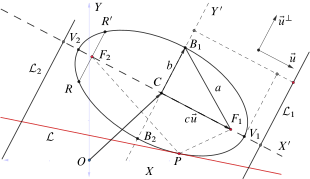
\includegraphics{elipse} 

}

\caption{Elipse}\label{fig:f1}
\end{figure}

\index{fff}
Sea la Tabla \ref{tab:ww} y la Figura \ref{fig:f1} entonces

\hypertarget{solucion-de-ecuaciones-diferenciales-mediante-la-trasformada-de-laplace}{%
\chapter{Solucion de ecuaciones diferenciales mediante la Trasformada de Laplace}\label{solucion-de-ecuaciones-diferenciales-mediante-la-trasformada-de-laplace}}

Example text outside R code here; we know the value of
pi is In this section, we give a very brief introduction to Pandoc's Markdown. Readers who are familiar with Markdown can skip this section. The comprehensive syntax of Pandoc's Markdown can be found on the Pandoc website \url{http://pandoc.org}.

\begin{quote}
``I thoroughly disapprove of duels. If a man should challenge me,
I would take him kindly and forgivingly by the hand and lead him
to a quiet place and kill him.''
\end{quote}

In this section, we give a very brief introduction to Pandoc's Markdown. Readers who are familiar with Markdown can skip this section. The comprehensive syntax of Pandoc's Markdown can be found on the Pandoc website \url{http://pandoc.org}. \(\sum_1^2\)

\begin{quote}
I thoroughly disapprove of duels. If a man should challenge me,
I would take him kindly and forgivingly by the hand and lead him
to a quiet place and kill him.

-- Mark Twain
\end{quote}

\[\begin{pmatrix}\alpha & \beta\\
\gamma & \delta
\end{pmatrix}-\frac{2}{3} \begin{pmatrix}\alpha_1 & \beta_2\\
\gamma & \delta
\end{pmatrix}\]
* La suma de dos matrices \(A_{n\times m}\) y \(B_{r\times s}\) \[A_{n\times m}\pm B_{n\times m}=[a_{ij}+b_{ij}]\]
* El producto de dos matrices \(A_{n\times m}\) y \(B_{r\times s}\) \[A_{n\times m}\cdot B_{n\times m}=[a_{ij}+b_{ij}]\]
\[X = \begin{bmatrix}1 & x_{1}\\
1 & x_{2}\\
1 & x_{3}
\end{bmatrix}\]

\[\begin{vmatrix}a & b\\
c & d
\end{vmatrix}=ad-bc\]

\[\begin{array}{ccc}
x_{11} & x_{12} & x_{13}\\
x_{21} & x_{22} & x_{23}
\end{array}\]

\hypertarget{appendix-apendice}{%
\appendix \addcontentsline{toc}{chapter}{\appendixname}}


\hypertarget{operadores-diferenciales-1}{%
\chapter{Operadores diferenciales}\label{operadores-diferenciales-1}}

Una suma de números representados por \(x_1, x_2, \ldots, x_n\) se simboliza en forma compacta mediante el simbolo \(\sum\) (sigma) es decir la suma de los números anteriores se puede escribir del siguiente modo \[x_1+x_2+\dots+x_n=\sum_{i=1}^nx_i.\]
Algunas propiedades son

\begin{enumerate}
\def\labelenumi{\arabic{enumi}.}
\tightlist
\item
  \(k\sum_{i=1}^nx_i=\sum_{i=1}^nkx_i\)
\item
  \(\sum_{i=1}^n\left(x_i+y_i\right)=\sum_{i=1}^nx_i+\sum_{i=1}^ny_i\)
\item
  \(\sum_{i=1}^nx_i\)
  \[\int_1^3=\lim_{n\to \infty}\sum_{i=0}^{n}f^i(x)\]
  citado por \citep{xie2015}
\end{enumerate}

\hypertarget{ee}{%
\section{ee}\label{ee}}

\hypertarget{eeeee}{%
\section{eeeee}\label{eeeee}}

\hypertarget{trasformada-de-laplace}{%
\chapter{Trasformada de Laplace}\label{trasformada-de-laplace}}

Una matriz es un arreglo de números distribuidos en filas y columnas por ejemplo la siguiente matriz
\[A=\begin{pmatrix}
a_{11}&a_{12}&\ldots&a_{1n}\\
a_{21}&a_{22}&\ldots&a_{2n}\\
\vdots & \vdots & \ddots &\vdots \\
a_{11}&a_{11}&\ldots&a_{nm}
\end{pmatrix}_{n\times n}\]
de \textbf{orden} \(n\times m\) tiene \textbf{entradas} \(a_{ij}\) donde el primer subindice indica la fila y el segundo la columna; es usual representar por simplicidad una matriz por \(A=[a_{ij}]_{n\times m}\). Si en el orden \(n=m\) entonces la matriz recibe el nombre de \textbf{matriz cuadrada} la suma de los elementos de la diagonal de una matriz cuadrada \(\sum_{i=1}^na_{ii}\) se llama \textbf{traza}\index{traza}. Si todas las \(a_{ij}\) son cero entonces la matriz \(A=0\) recibe el nombre matriz \textbf{nula}.

Dos matrices son iguales si tienen el \textbf{mismo orden} y cada una de las entradas respectivas son iguales es decir \(A=[a_{ij}]_{n\times m}\) y \(B=[b_{ij}]_{n\times m}\) son iguales si \(a_{ij}=b_{ij}\), \(i=1,2,\ldots n\) y \(j=1,2,\ldots m\)

\hypertarget{algebra-de-matrices}{%
\section{Algebra de matrices}\label{algebra-de-matrices}}

Sean las matrices \(A=[a_{ij}]_{n\times m}\) y \(B=[b_{ij}]_{p\times q}\) entonces la suma y producto de matrices se definen

\begin{enumerate}
\def\labelenumi{\arabic{enumi}.}
\item
  Sea \(k\) un escalar entonces se verifica que \(kA=[ka_{ij}]\), \(i=1,2,\ldots n\) y \(j=1,2,\ldots m\) es decir el escalar \(k\) multiplica a cada una de las entradas de la matriz.
\item
  La suma o diferencia es posible si \(n=p\) y \(m=q\) es decir los ordenes de \(A\) y \(B\) son iguales, entonces la suma o diferencia resulta \(A\pm B=[a_{ij}+b_{ij}]_{n\times m}\), \(i=1,2,\ldots n\) y \(j=1,2,\ldots m\)
\item
  El producto es posible si \(m=p\) es decir el número columnas de la primera matriz es igual al número de filas de la segunda matriz, el orden de la matriz resultante es \(n\times q\) además
  \begin{align*}
  A\cdot B&=\left[\sum_{k=1}^pa_{ik}b_{kj}\right]_{n\times q}\\
  &=\begin{pmatrix}
  \sum_{k=1}^ma_{1k}b_{k1}&\sum_{k=1}^ma_{1k}b_{k2}&\ldots&\sum_{k=1}^ma_{1k}b_{kq}\\
  \sum_{k=1}^ma_{2k}b_{k1}&\sum_{k=1}^ma_{2k}b_{k2}&\ldots&\sum_{k=1}^ma_{2k}b_{kq}\\
  \vdots & \vdots & \ddots &\vdots \\
  \sum_{k=1}^ma_{nk}b_{k1}&\sum_{k=1}^ma_{nk}b_{k2}&\ldots&\sum_{k=1}^ma_{nk}b_{kq}\\
  \end{pmatrix}_{n\times q}
  \end{align*}
\end{enumerate}

donde \(i=1,2,\ldots n\) y \(j=1,2,\ldots m\)

\BeginKnitrBlock{example}
\protect\hypertarget{exm:unnamed-chunk-15}{}{\label{exm:unnamed-chunk-15} }Sean \(\begin{pmatrix} 3&-1&2\\ 2&-1&2\\ 1&-1&0\\ 5&0&0\\ \end{pmatrix}_{4\times 3}\) y \(\begin{pmatrix} 0&-1&2&2&0\\ 1&-1&-2&1&1\\ 3&-1&-3&5&2\\ \end{pmatrix}_{3\times 5}\) entonces \(A\cdot B=\begin{pmatrix} 5&-4&2&15&3\\ 5&-3&0&13&3\\ -1&0&4&1&-1\\ 0&-5&10&10&0\\ \end{pmatrix}_{4\times 5}\)
\EndKnitrBlock{example}

En caso de ser posible la multiplicación entre \(A\), \(B\) y \(C\) entonces se verfican las siguientes propiedades

\begin{itemize}
\tightlist
\item
  \(A(B+C)=AB+AC\)
\item
  \((A+B)C\)
\item
  \(A(BC)=(AB)C\)
\end{itemize}

\bibliography{book.bib,packages.bib}

\printindex

\end{document}
